\documentclass[a4paper]{report}
\usepackage{graphicx}
\usepackage[utf8]{inputenc}
\usepackage{xcolor} % Load this before hyperref
\definecolor{softblue}{RGB}{70,130,180}
\usepackage[colorlinks=true, linkcolor=softblue, citecolor=softblue, filecolor=softblue, urlcolor=softblue]{hyperref}
\usepackage{url}

\title{Design \& Architecture of Erbut, An Elegant Web Based Linkfolio}
\author{
    Yazeed AlKhalaf \\
    Khalil Melhem \\
    Khaled Hazzam \\
    \textbf{Course:} SWE 302 - Software Design \& Architecture \\
    \textbf{Instructor:} Dr. Ahmed Ghoneim
}
\date{12 Feb, 2024}

\begin{document}

\maketitle

\newpage

\tableofcontents

\chapter*{Abstract}

Erbut presents a dynamic, web-based platform enabling users to create and manage personalized 'Erbuts'—elegant linkfolios showcasing a curated list of links. These linkfolios, hosted as subdomains on erbut.me or linked to custom domains, offer a unique way to display online presence.

Additionally, users can integrate Google Analytics for enhanced data collection. The subscription model, facilitated via Stripe, unlocks premium features, enhancing user experience and customization. Erbut stands out as a versatile solution for creating and monitoring professional and personal online portfolios and brands.

This paper extensively explores the design and architecture of Erbut, focusing on its robust, scalable backend and user-friendly frontend. It highlights the integration of technologies for domain management, analytics, and payment processing, emphasizing the platform's efficiency and security.

\newpage

\chapter{System Overview}

This section will showcase the system from an internal point of view. Using UML diagrams to draw the system, reading this section should allow the reader to understand how the system is built on a high level.

\section{Big Picture}

\begin{figure}[h!]
    \centering
    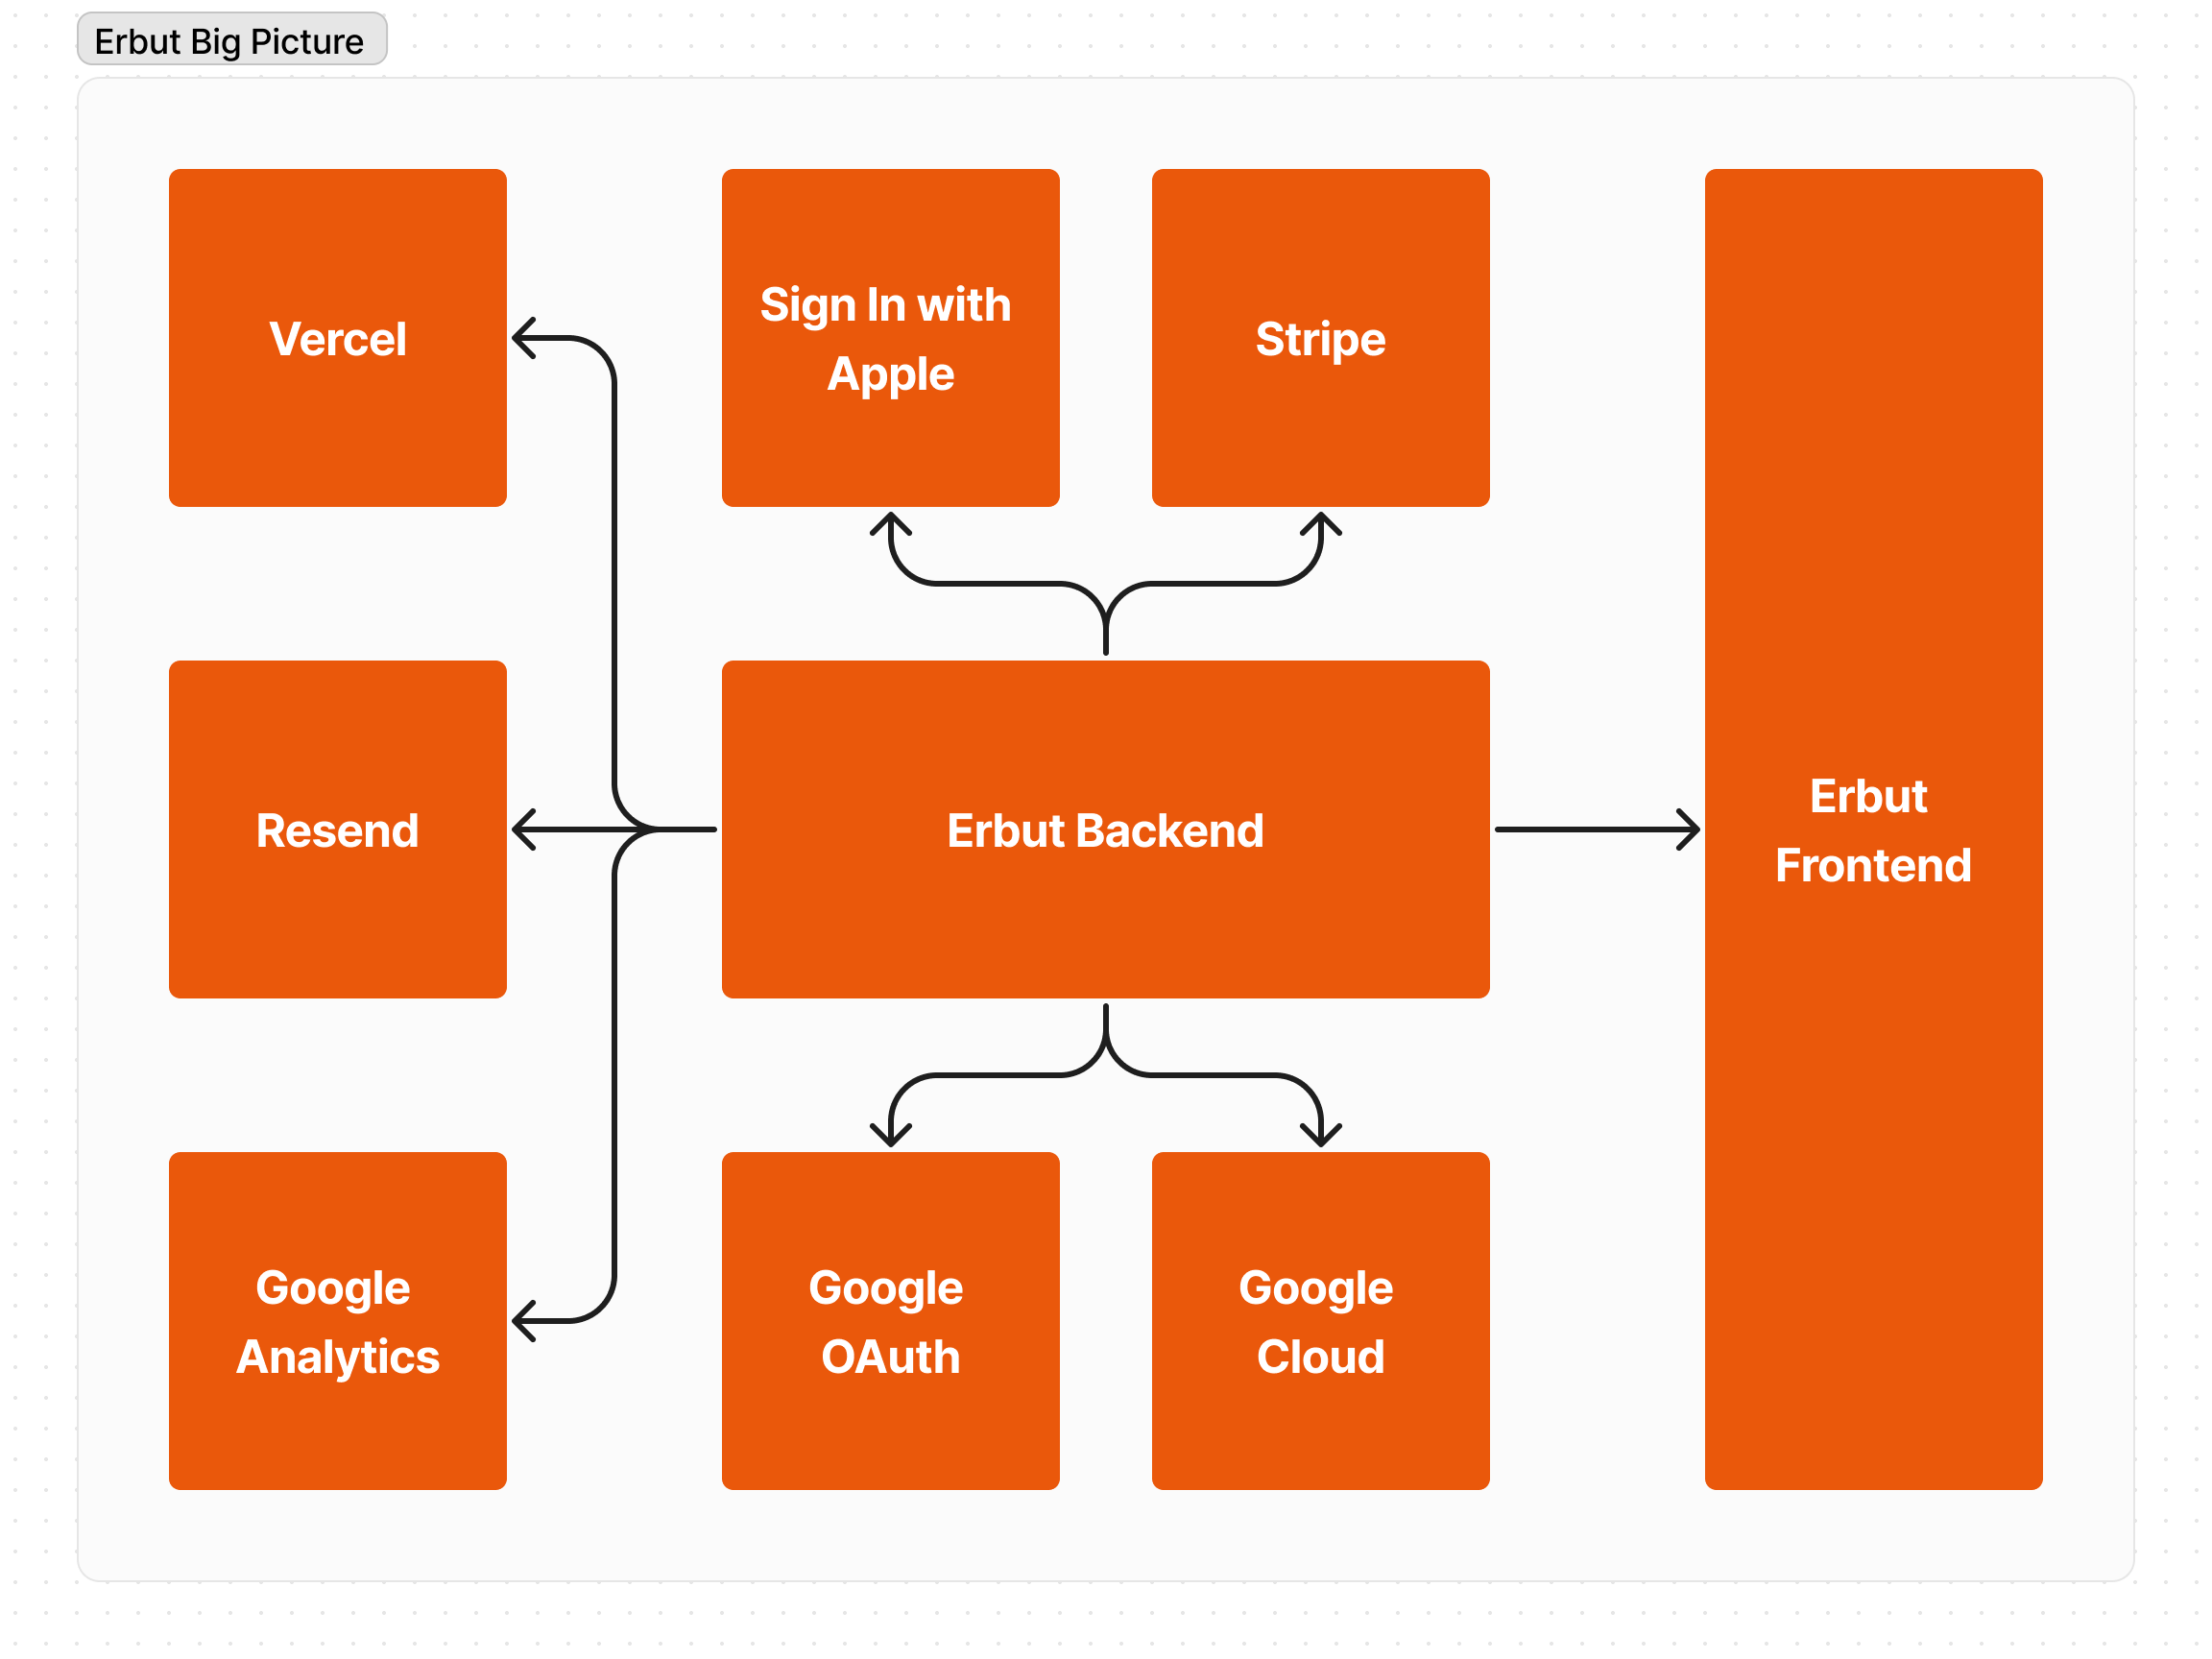
\includegraphics[width=0.8\textwidth]{images/erbut-big-picture.png}
    \caption{Big Picture Diagram of Erbut}
    \label{fig:bigpicture}
\end{figure}

The Big Picture diagram sketch seen in Figure \ref{fig:bigpicture} provides a high-level overview of Erbut’s system architecture, highlighting its backend central to operations, integrating with services like Vercel, Stripe, Resend, Sign in with Apple, Google OAuth, Google Cloud, and Google Analytics.

\section{Abstract View}

\begin{figure}[h!]
    \centering
    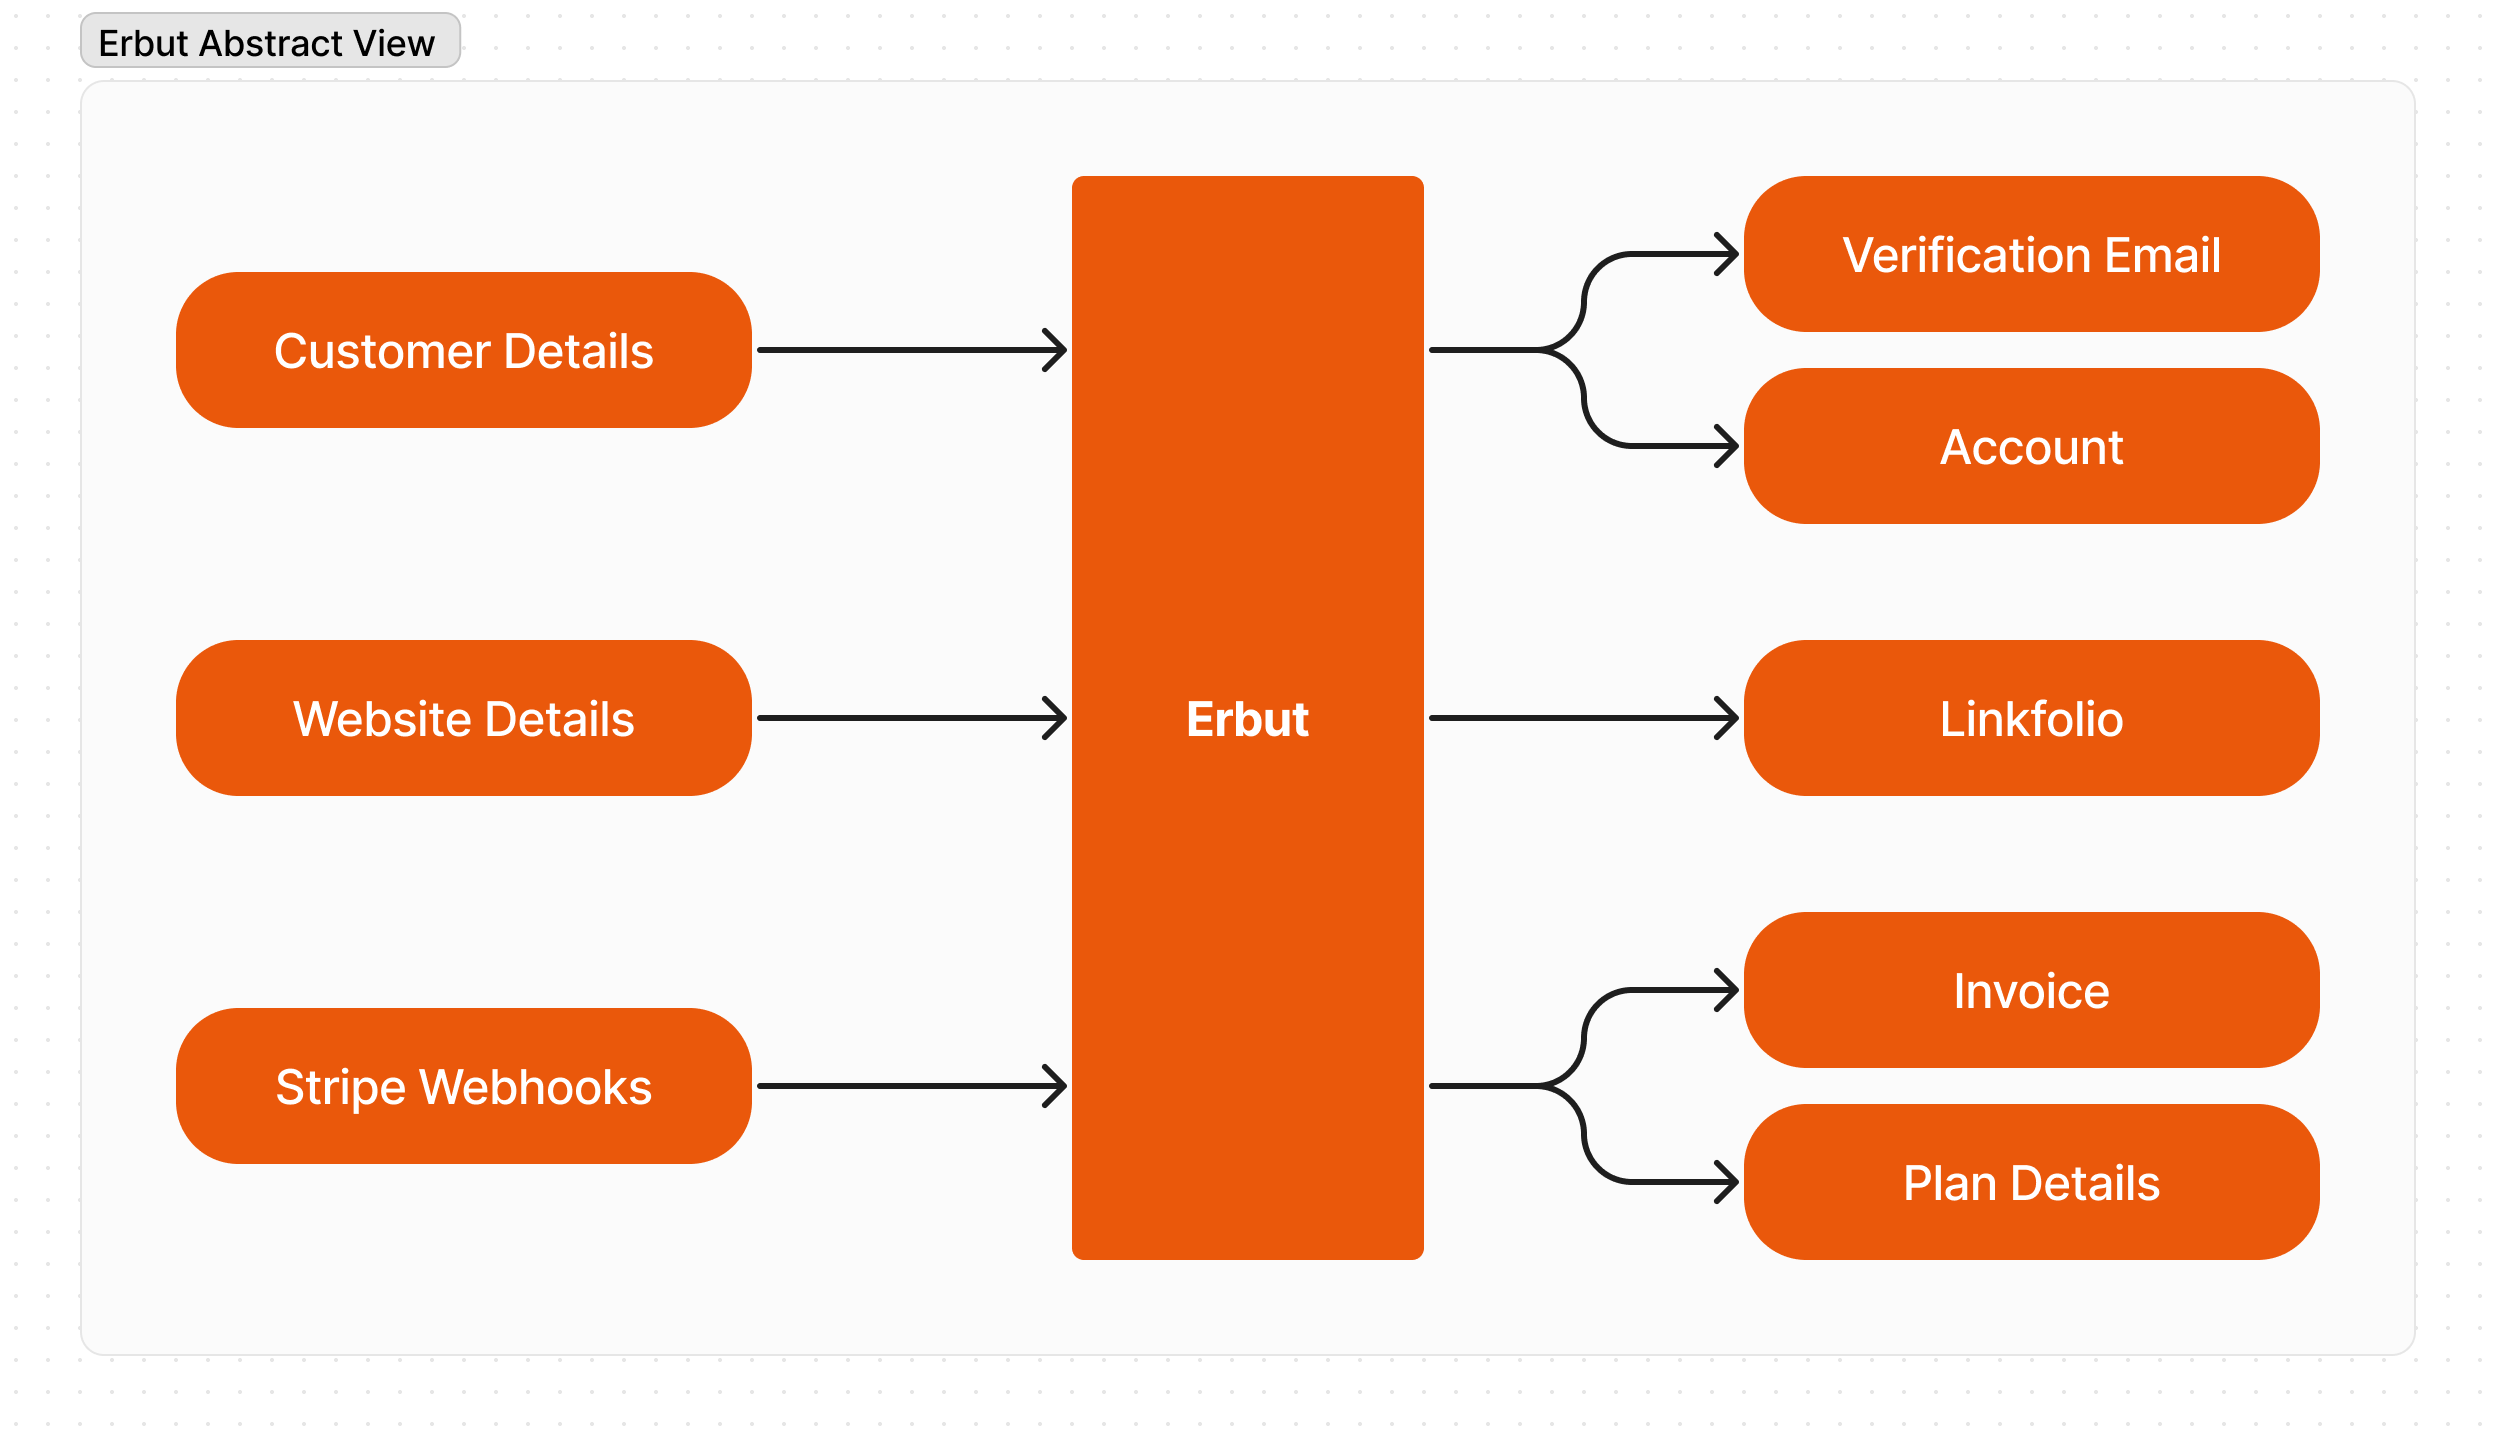
\includegraphics[width=0.8\textwidth]{images/erbut-abstract-view.png}
    \caption{Black Box Diagram of the System}
    \label{fig:abstractview}
\end{figure}

The abstract view diagram seen in Figure \ref{fig:abstractview} helps us understand the inputs the system requires and the outputs it will produce. A glance at the diagram shows that we use Customer Details to create an account initially and then to verify the user's identity in subsequent interactions. Website Details are used to construct the Erbut Linkfolio. Additionally, Stripe webhooks provide real-time information about our users’ subscription statuses.

\section{Subsystem View}

\begin{figure}[h!]
    \centering
    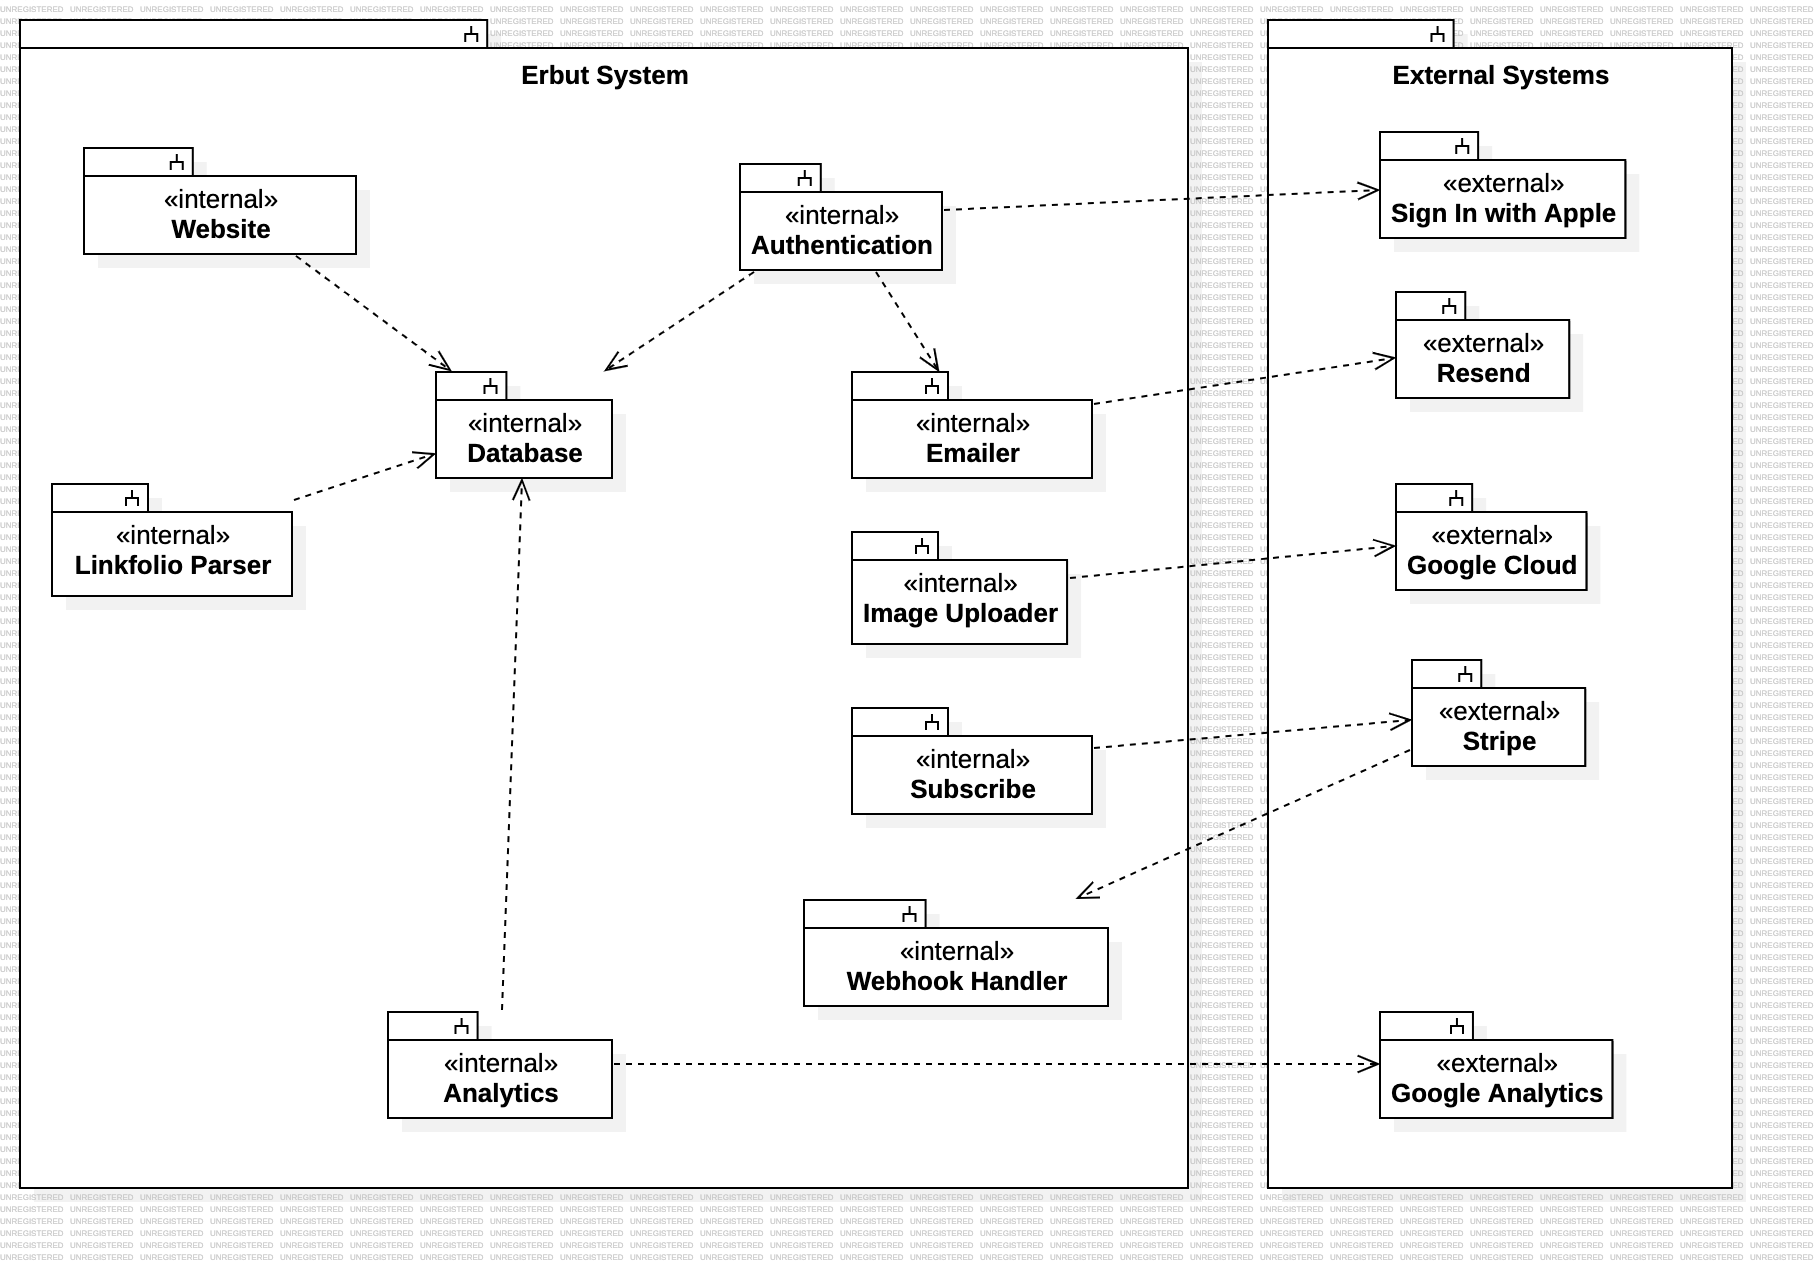
\includegraphics[width=0.8\textwidth]{images/erbut-package-diagram.png}
    \caption{Package Diagram of Erbut}
    \label{fig:subsystemview}
\end{figure}

The subsystem diagram found below in Figure \ref{fig:subsystemview} represents all the components that our system (Erbut) consists of internally and externally. External subsystems represent the components we are using directly without building them from scratch. On the other hand, internal subsystems are built by us from the ground up.

\chapter{Functionalities of The Subsystems}

This section highlights the description of the sub-systems previously presented in the Sub-System View of Erbut.

\section{Database (\texttt{internal})}

Stores the data for the system, such as our customers’ details and their website data.

\section{Authentication (\texttt{internal})}

Responsible for the authentication of users whether it’s their first time accessing the system or a regular user. Integrates with Google OAuth and Sign in with Apple to offer more authentication options.

\section{Website (\texttt{internal})}

API for the front-end to allow the customer to create and manage websites (Erbuts).

\section{Linkfolio Parser (\texttt{internal})}

It fills out the template of the Erbut based on the data in the database. It knows which Erbut to query by its subdomain. It then parses the template and fills it with data, then finally returns it to the client.

\section{Emailer (\texttt{internal})}

This service is responsible for sending emails. Other systems like Authentication depend on it to send verification and reset password emails. It accepts email and a template id.

\section{Image Uploader (\texttt{internal})}

This service allows customers to upload an image and get a URL for it. This is helpful to put images in their Erbuts by hosting it on our servers.

\section{Subscribe (\texttt{internal})}

This service allows the customer to manage their billing information and subscribe or change their plan.

\section{Webhook Handler (\texttt{internal})}

This service allows Stripe, our payment gateway, to send us updates about our customers' billing state. Whether they are subscribed, paid, did not pay, or even are late on payment.

\section{Analytics (\texttt{internal})}

This service collects and aggregates data from the Erbuts and saves it for our customers to view and take decisions based on it.

\section{Google Analytics (\texttt{external})}

Collects and analyzes data of visitors and their behaviors when visiting a customer’s Erbut (Linkfolio).

\section{Google Cloud (\texttt{external})}

Responsible for providing computing resources, data storage, and hosting the system backend services. It’s a cloud computing service that runs on the same infrastructure that Google uses for its own products.

\section{Stripe (\texttt{external})}

Responsible for handling all payment transactions, including processing customer credit cards, managing secure payment information, and handling subscription billing services.

\section{Resend (\texttt{external})}

Responsible for automated email communications, such as account verification, notification, and other automated email responses based on user actions or system triggers.

\chapter{Data Flow of Erbut}

\section{Batch Sequential}

\begin{figure}[h!]
    \centering
    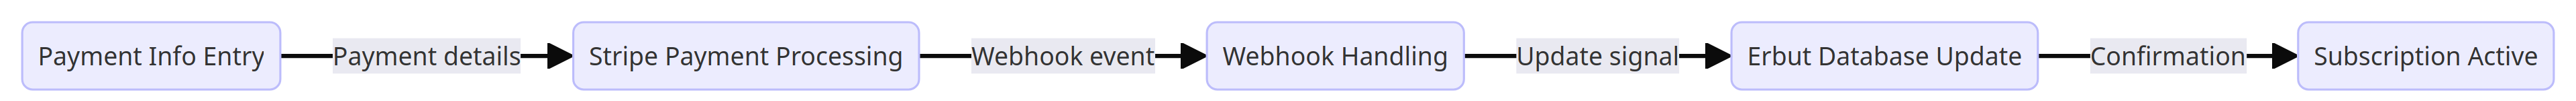
\includegraphics[width=0.8\textwidth]{images/data-flow/user-subscription-batch-sequential.png}
    \caption{Batch Sequential of Website Creation}
    \label{fig:batch-sequential-user-subscription}
\end{figure}

In Figure \ref{fig:batch-sequential-user-subscription} above, the diagram shows how the data in the subscription process of Erbut. Below are the steps explaining how and when the interactions in the diagram happens:

\begin{enumerate}
    \item The Payment Info is entered and Payment Details are extracted from it.
    \item The Payment Details are now an input to the Stripe Payment Processing, which is an external system, and the output is is a webhook event.
    \item The webhook event is now an input to the Webhook Handler, which is an internal system of Erbut, and the output is an update signal for the database.
    \item The update signal for the database is now an input to the Database, which is an internal system of Erbut, and the output is a confirmation signal.
    \item The confirmation signal shows that the subscription is active now.
\end{enumerate}

\section{Pipe and Filter}

\begin{figure}[h!]
    \centering
    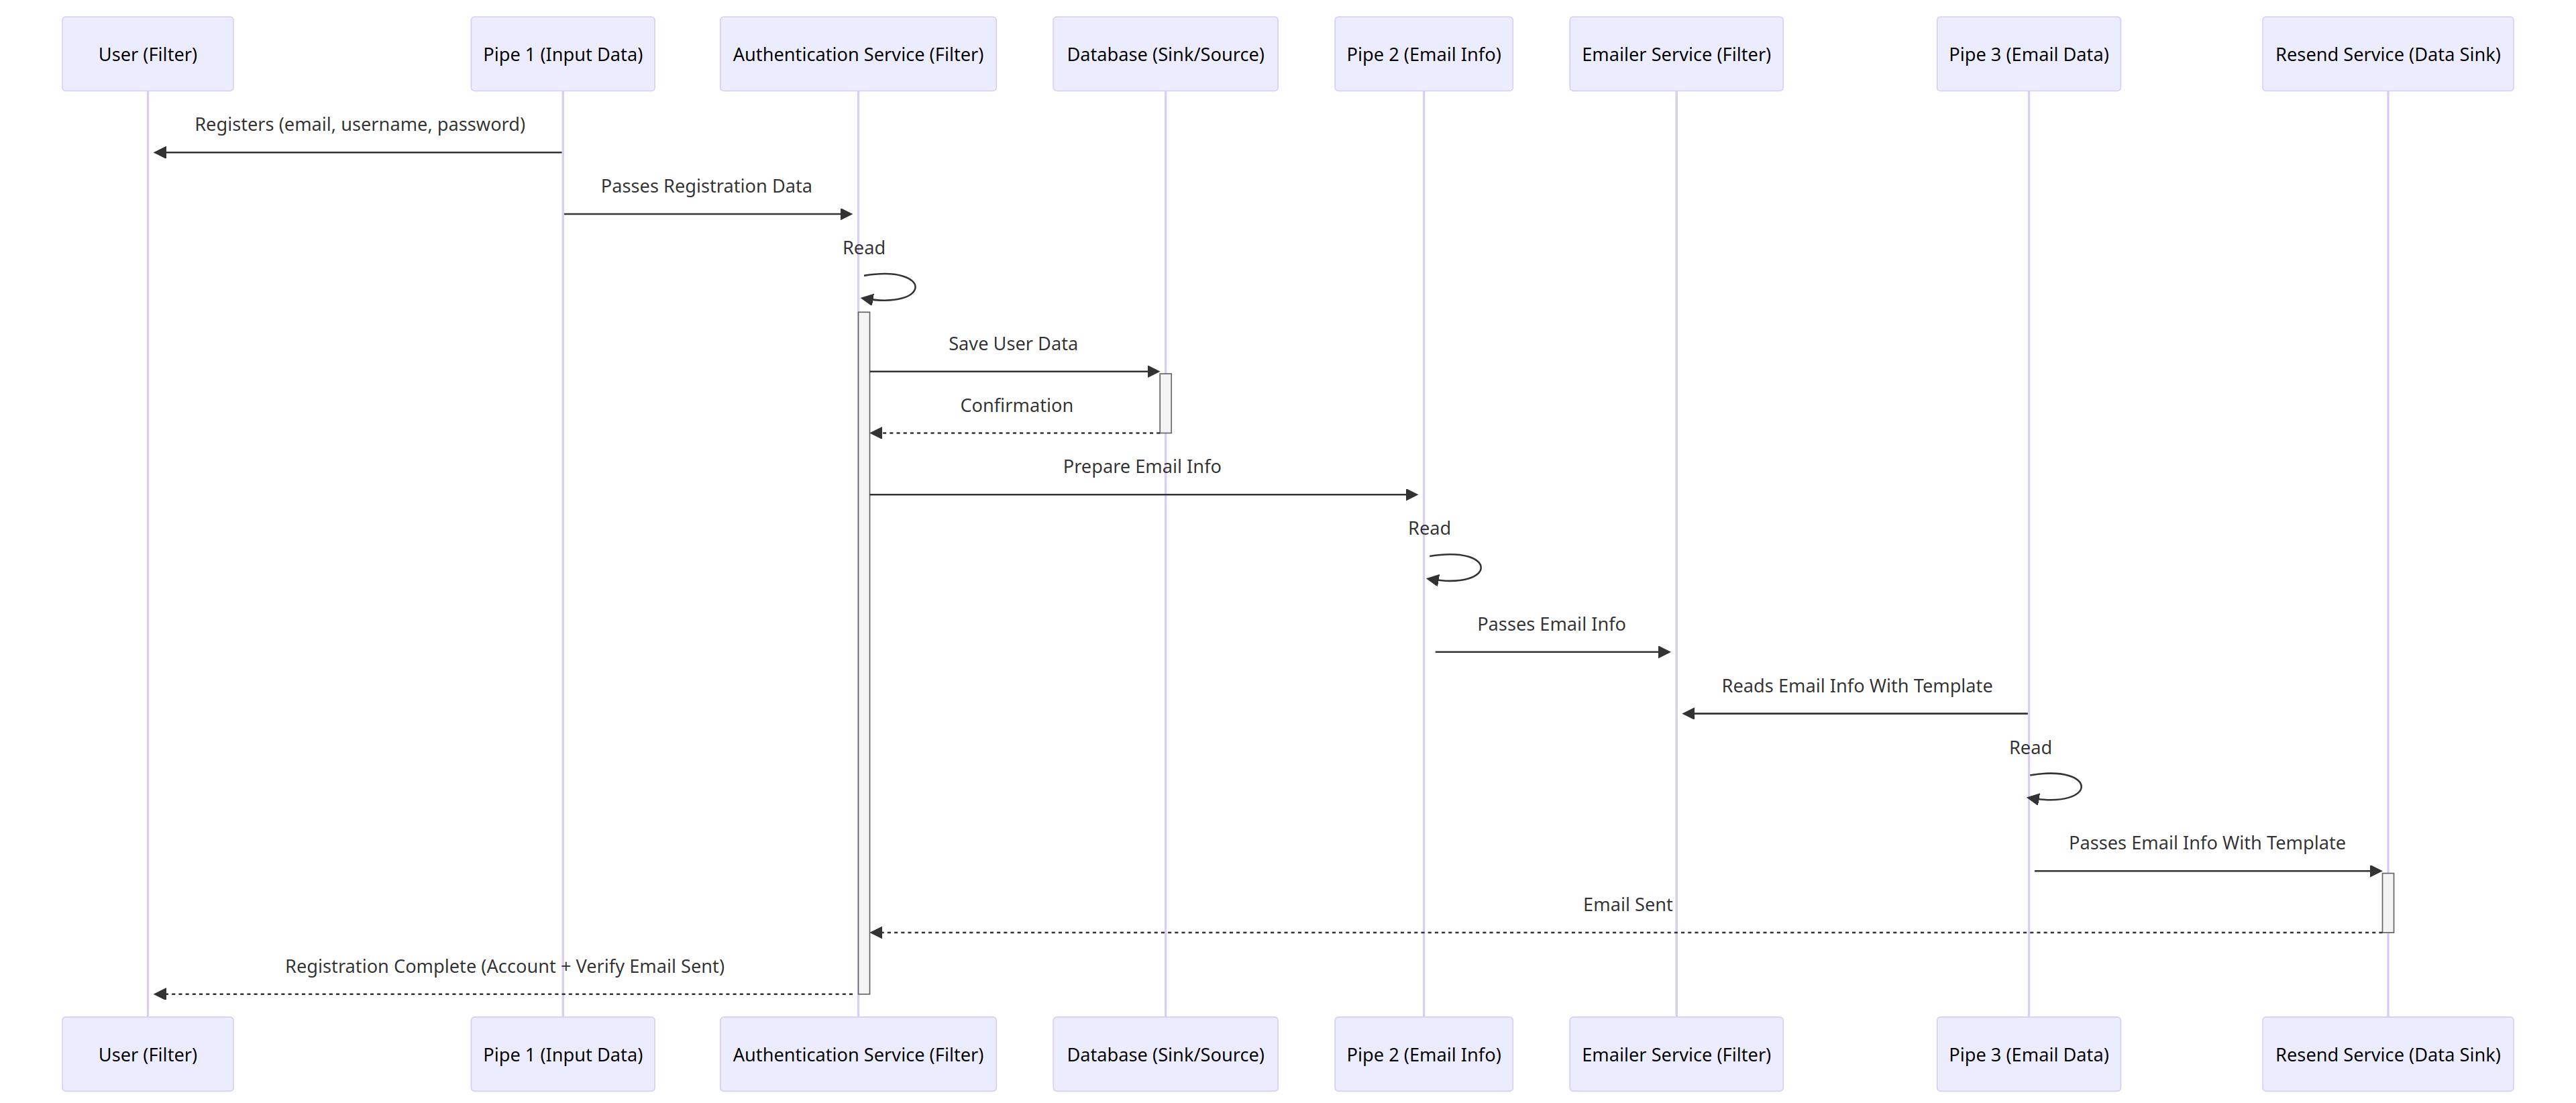
\includegraphics[width=0.8\textwidth]{images/data-flow/registration-pipe-and-filter.png}
    \caption{Pipe and Filter of User Registration}
    \label{fig:pip-and-filter-user-registration}
\end{figure}

In Figure \ref{fig:pip-and-filter-user-registration} below, the diagram shows how the data in the registration process of Erbut flows from one sub system to another. Below are the steps explaining how and when the interactions in the diagram happens:

\begin{enumerate}
    \item The Input Data pipe reads the email, username, and password from the User filter and then writes this registration data to the Authentication Service filter.
    \item Then the Authentication Service filter reads the passed registration data and writes it to the Database, and waits for confirmation.
    \item Once the confirmation is received, the Authentication Service filter writes the Email Info to the Email Info pipe.
    \item The Email Info pipe reads the email and writes it to the Emailer filter.
    \item The Email Data pipe reads the Email Info with Template and writes it to the Resend Service filter, which is our data sink.
\end{enumerate}

\chapter{Repository Diagram}

\begin{figure}[h!]
    \centering
    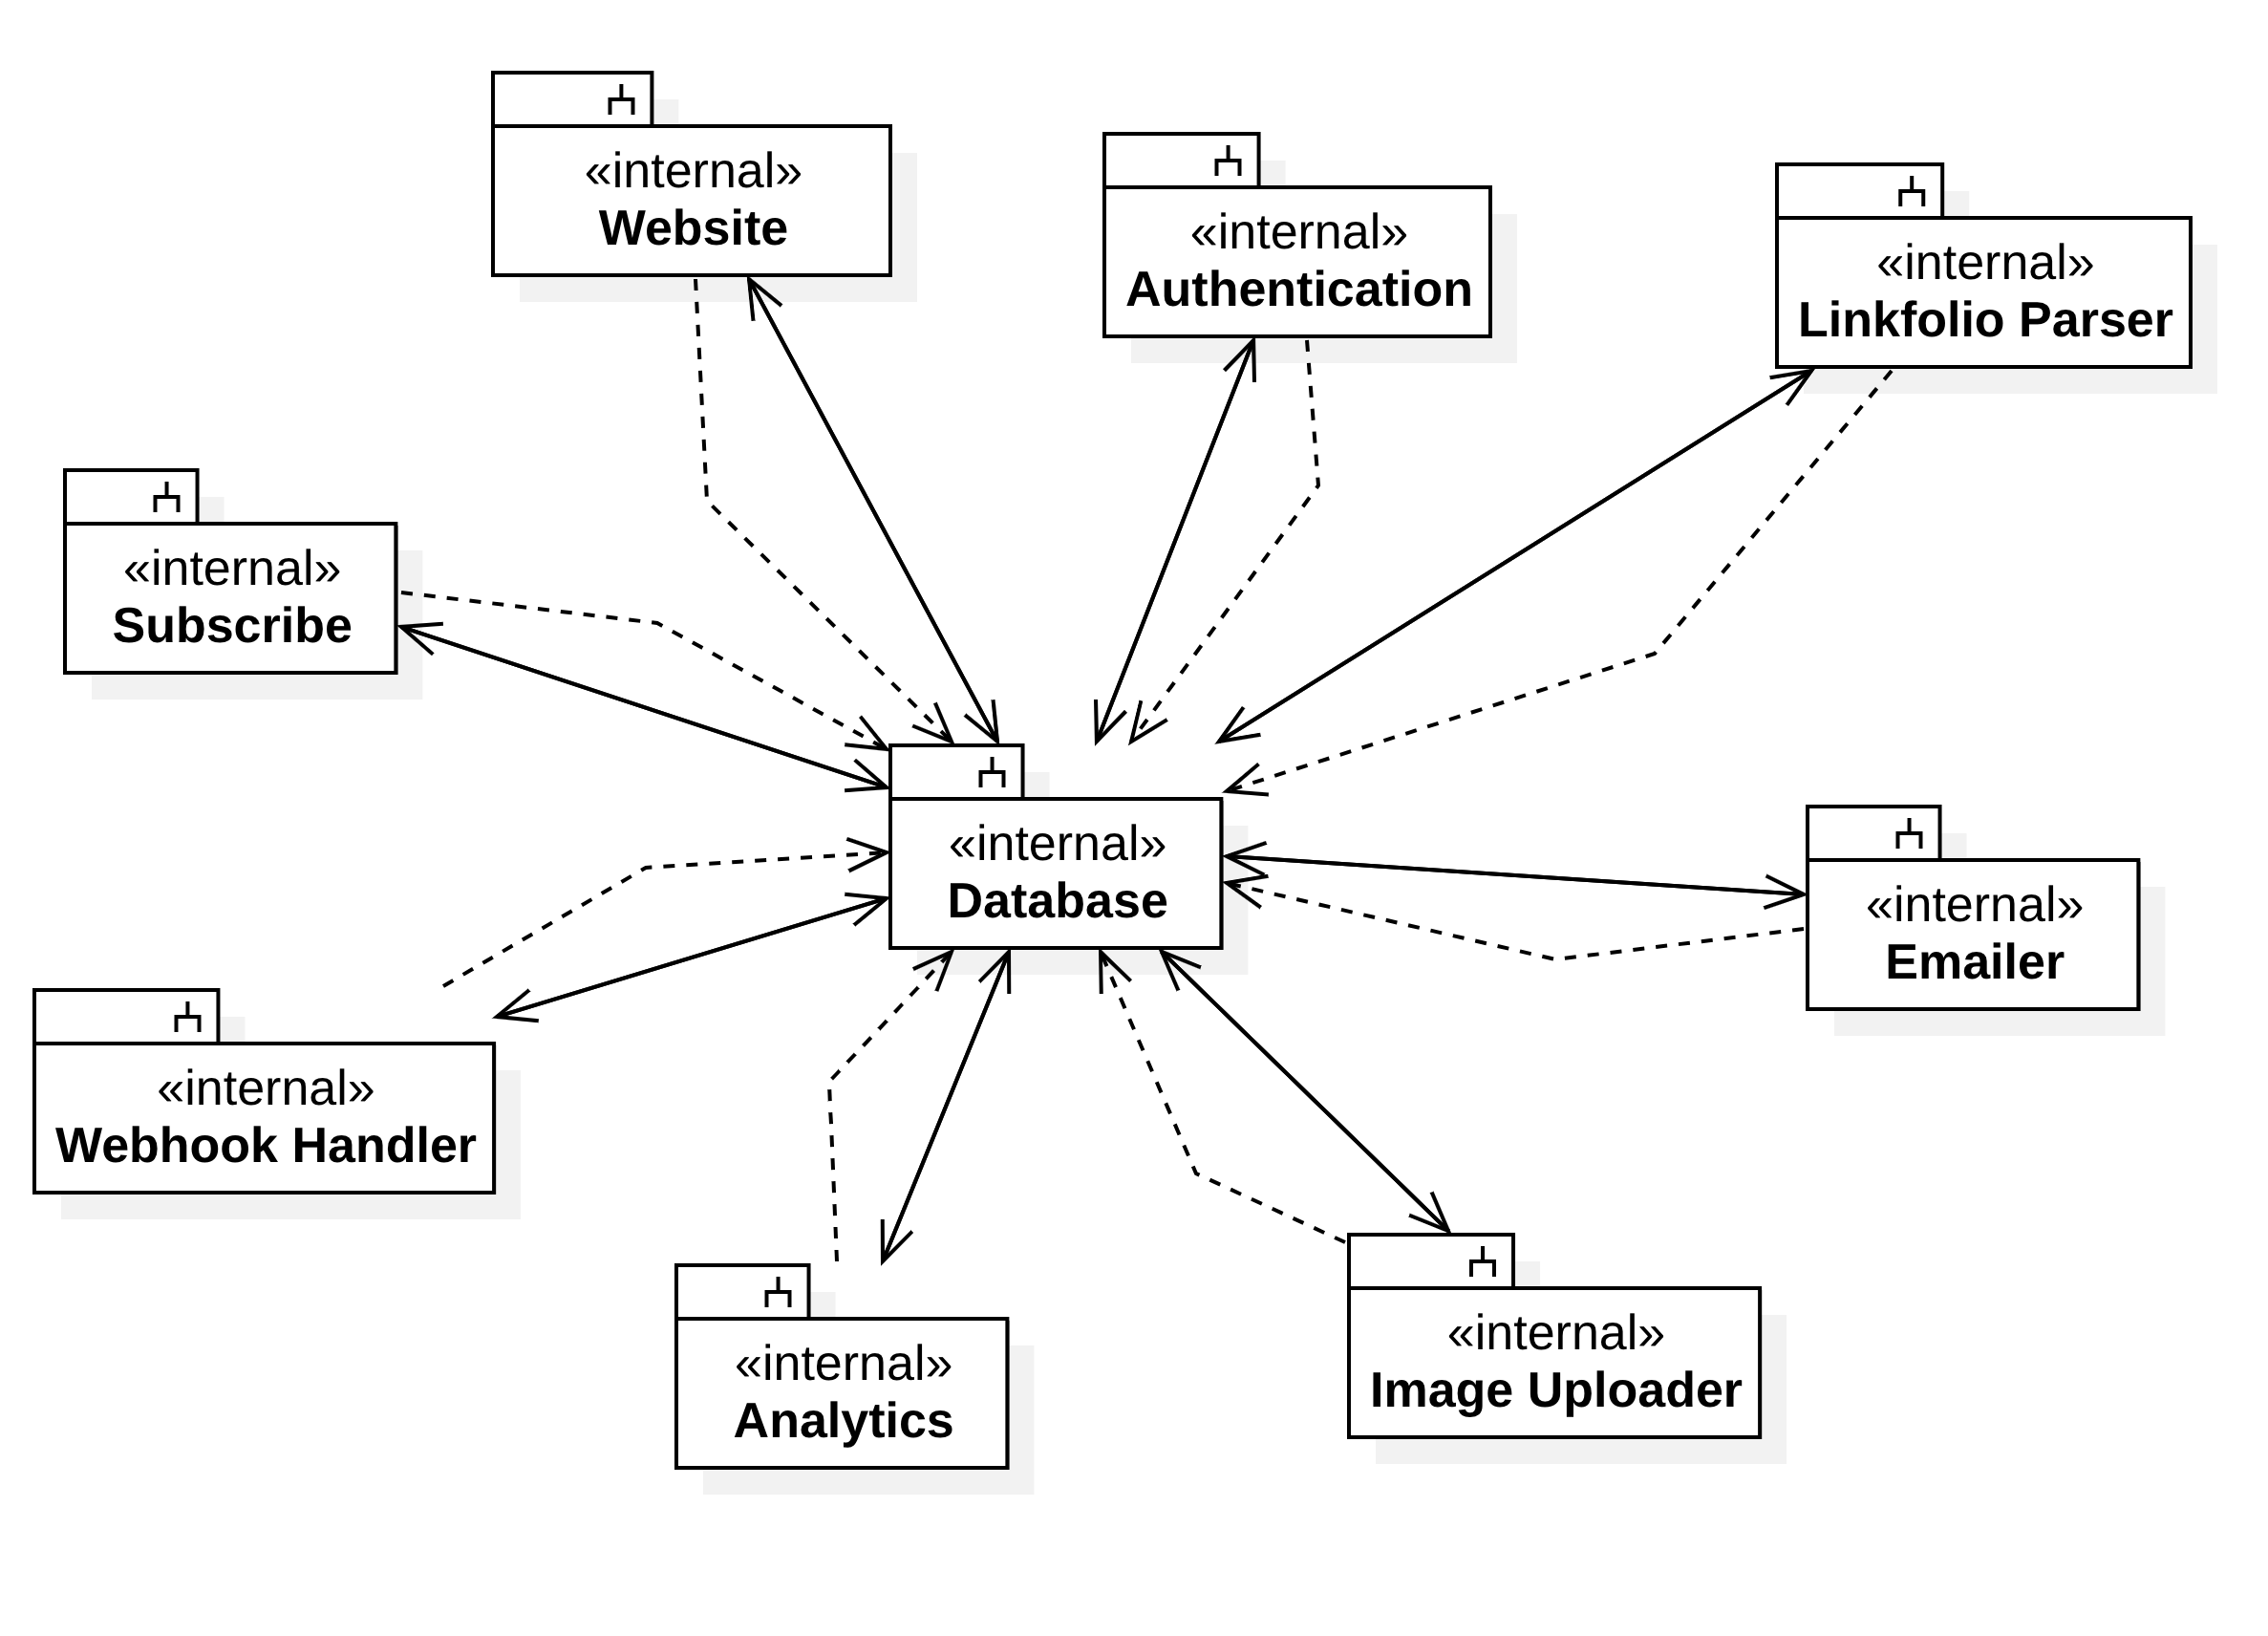
\includegraphics[width=0.8\textwidth]{images/erbut-repository-diagram.png}
    \caption{Repository Diagram of Erbut}
    \label{fig:repository-diagram}
\end{figure}

The Repository Diagram of Erbut, shown in Figure \ref{fig:repository-diagram}, illustrates the system's centralized data management structure, highlighting how different subsystems interact with the central repository. This visual representation underscores the central database's role as the core repository where all data is stored and accessed, ensuring data consistency and integrity across the system.

\begin{enumerate}
    \item \textbf{Central Database (Repository)}: The primary storage for all data related to users, their linkfolios, subscription information, and analytics, acting as the single source of truth.
    \item \textbf{Authentication System}: Retrieves and verifies user credentials from the central database, managing secure login processes and session tokens.
    \item \textbf{Website Management System}: Utilizes the central database to manage data related to user-created linkfolios, including layouts, links, and custom domains.
    \item \textbf{Subscription Management System}: Manages user subscription details and interfaces with external systems like Stripe to process transactions and update subscription statuses.
    \item \textbf{Analytics System}: Stores and analyzes data on user interactions with linkfolios, providing insights into performance based on information stored in the central database.
    \item \textbf{Email Communication System}: Sends automated emails for various user notifications, accessing contact information from the central database to ensure accuracy.
    \item \textbf{External Integration Points}: Includes connections to services like Stripe and Google Analytics, synchronizing data with the central database for cohesive system functionality.
\end{enumerate}

This diagram emphasizes the significance of the central database in facilitating efficient data flow and interaction between subsystems and external services, ensuring the Erbut platform operates cohesively.

\chapter{Architecture}

The architecture of Erbut is elegant and scalable, designed to accommodate the platform's dynamic and user-centric functionalities. The system's architecture is based on a layered structure, ensuring a clear separation of concerns and modularity. The layered architecture diagram showcases the system's presentation, application, and data layers, each responsible for specific functionalities.

\section{Layered Architecture}

\begin{figure}[h!]
    \centering
    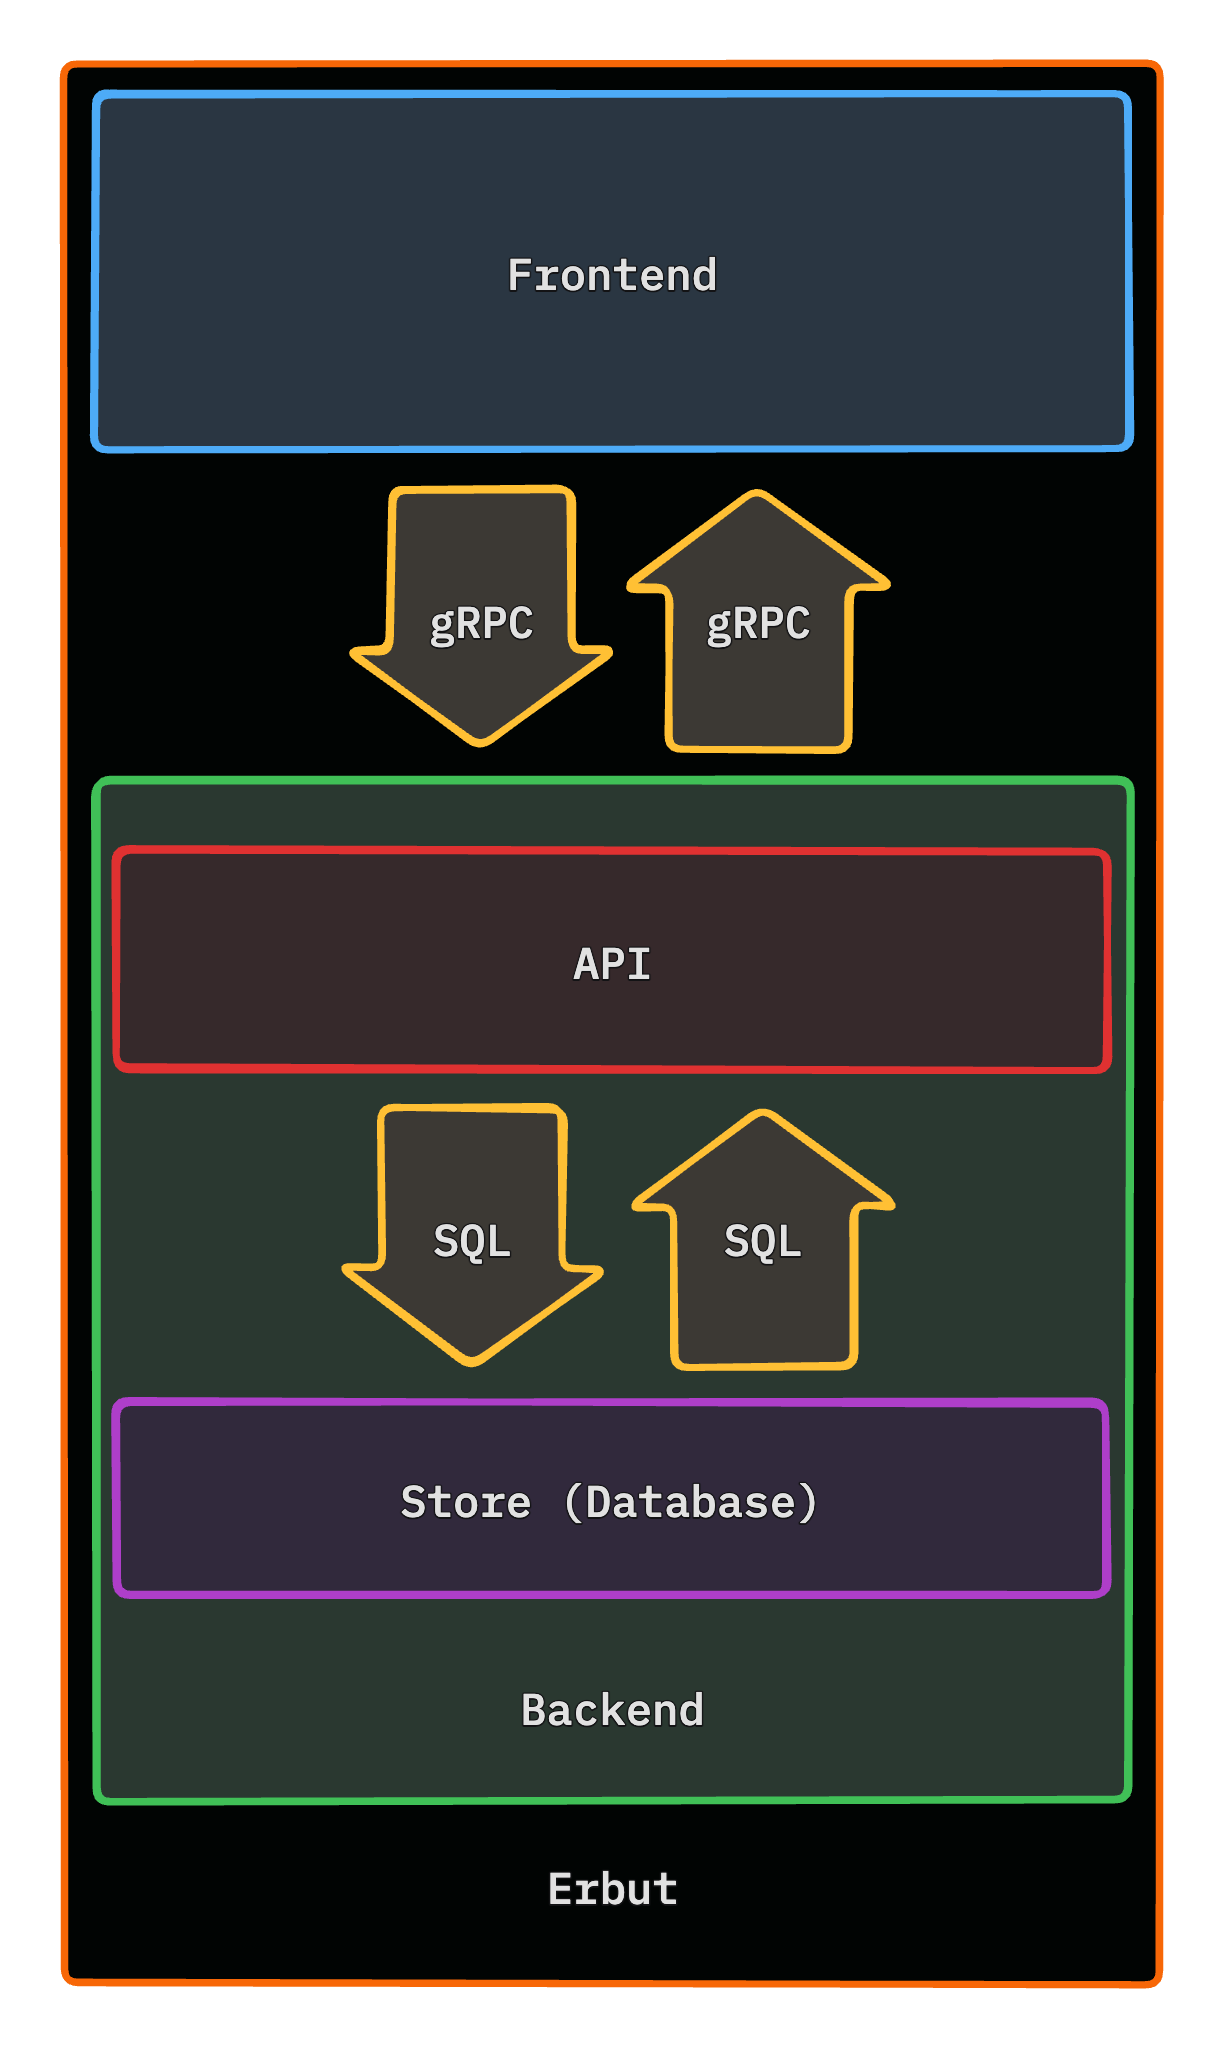
\includegraphics[width=0.8\textwidth]{images/erbut-layered-architecture.png}
    \caption{Layered Architecture of Erbut}
    \label{fig:layered-architecture}
\end{figure}

In the Layered Architecture diagram shown in Figure \ref{fig:layered-architecture}, the system is divided into 3 layers, each responsible for specific functionalities. The frontend is the layer that the user interacts with. It is built in React. The frontend communicates with the backend through an API. This API is a gRPC API. The backend is built in Go. The backend communicates with the database, which is a PostgreSQL database. So the communication happens through SQL.

\section{MVC Architecture}

\textbf{MVC} stands for \textbf{M}odel \textbf{V}iew \textbf{C}ontroller. In our system, Erbut, we use MVC on the frontend that is build in React. We use \href{https://www.npmjs.com/package/zustand}{Zustand} for state management. The Model is the data that the user interacts with. The View is the UI that the user interacts with. The Controller is the logic that connects the Model and the View.

The MVC architecture is as follows:
\begin{itemize}
    \item The Controller is the Zustand store.
    \item The View is the React components.
    \item The Model is the data that the Zustand store holds.
\end{itemize}

\begin{figure}[h!]
    \centering
    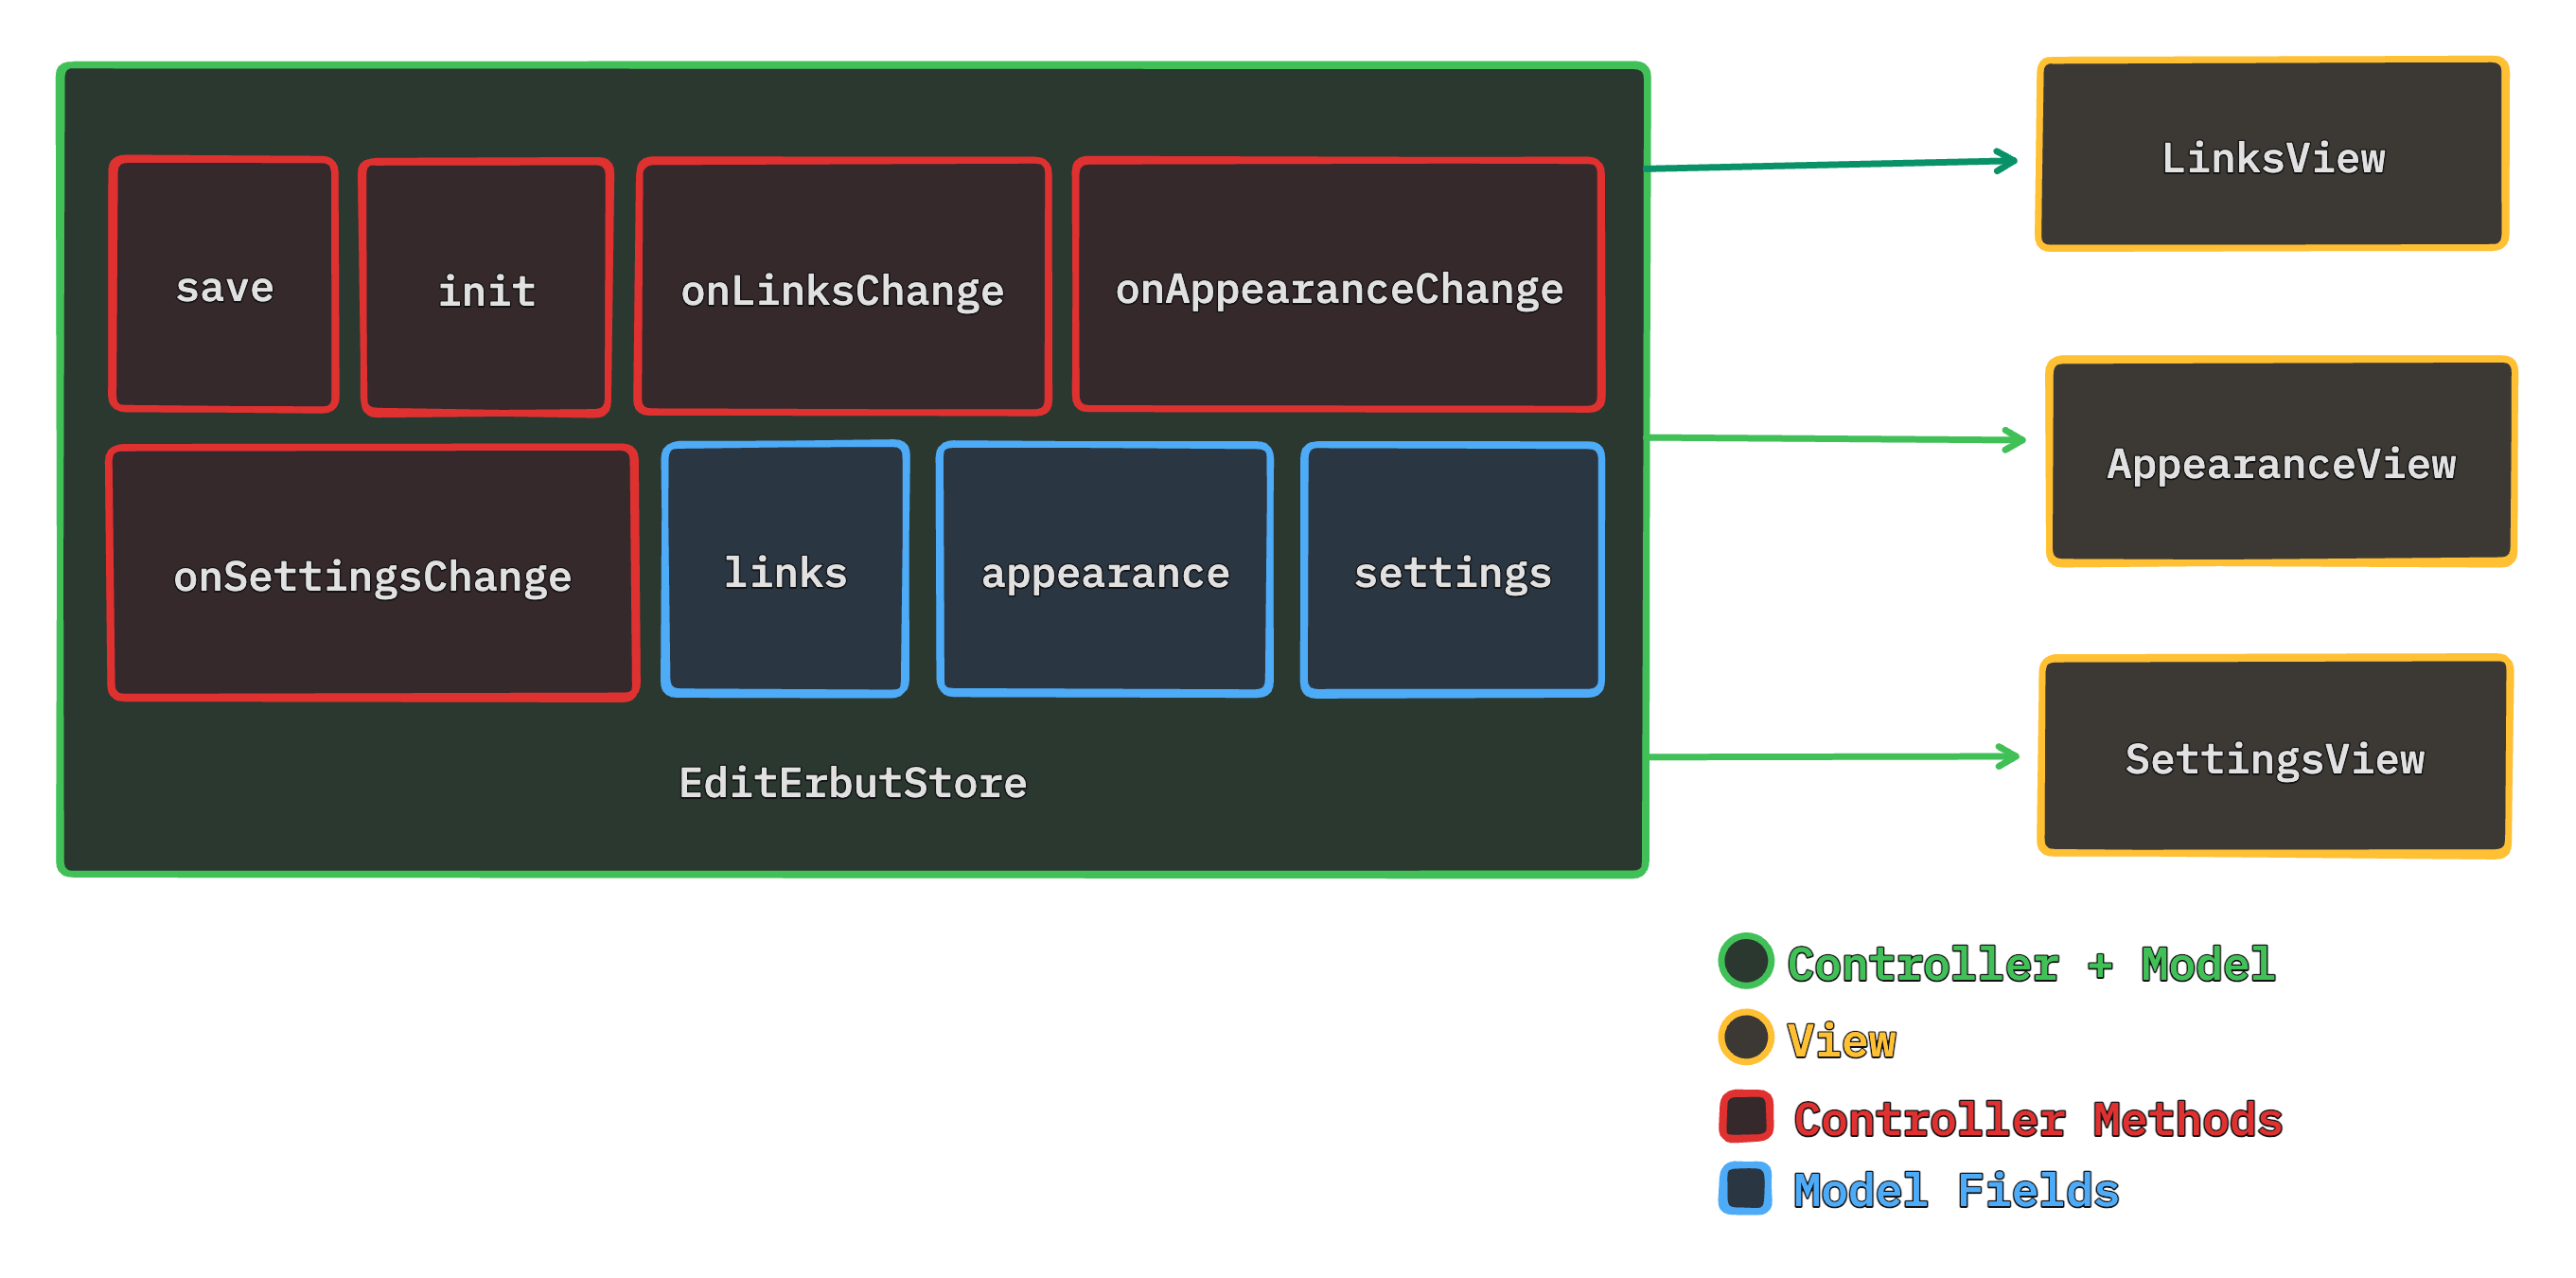
\includegraphics[width=0.8\textwidth]{images/erbut-mvc.png}
    \caption{MVC Example from Erbut}
    \label{fig:mvc-example}
\end{figure}

\end{document}
